\documentclass{standalone}

\usepackage{tikz}
\usepackage{pgfplots}
\begin{document}
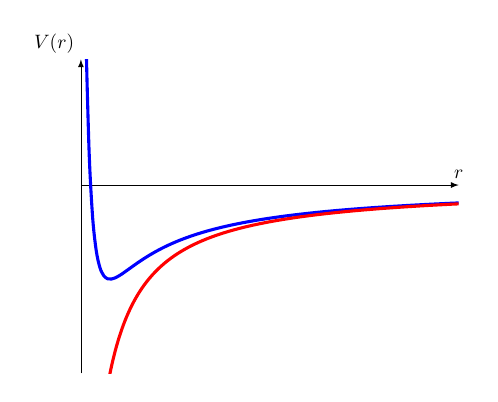
\begin{tikzpicture}[scale=0.7] % Reduce la escala al 70%
    \begin{axis}[
        xmin=0.5, xmax=20, % Establece el rango del eje x
        ymin=-1.5, ymax=1, % Ajusta el rango para el eje y
        smooth,
        samples=100,
        tick style={draw=none}, % Oculta los tics de los ejes
        xtick=\empty, % Elimina los números del eje x
        ytick=\empty, % Elimina los números del eje y
        axis lines=middle,
        axis line style={-latex}, % Flechas en los ejes
        xlabel={$r$},
        ylabel={$V(r)$},
        xlabel style={at={(axis description cs:1.0,0.6)}, anchor=south}, % Debajo de la flecha del eje x
        ylabel style={at={(axis description cs:0,1.05)}, anchor=east} % A la izquierda de la flecha del eje y
    ]
    \addplot[blue, ultra thick, domain=0.5:20] {3*(1/x^2-1/x)};
    \addplot[red, ultra thick, domain=0.5:20] {-3/x)};
    
    \end{axis}
    \end{tikzpicture}
\end{document}